% Compiler: LaTeX => PDF

\documentclass[xcolor=dvipsnames]{beamer}

\mode<presentation>
{
	\usetheme{BerlinHUB}
	%\setbeamercovered{transparent}
}

\usepackage[ngerman]{babel}
\usepackage[utf8]{inputenc}

\usepackage{helvet}
\usepackage[T1]{fontenc}

%\usepackage{multimedia}
%\usepackage{graphicx}
%\usepackage[nolist]{acronym}

%\usepackage{stackengine}
%\usepackage{array}

%\usepackage{enumitem}

%\setitemize{label=\usebeamerfont*{itemize item}%
%  \usebeamercolor[fg]{itemize item}
%  \usebeamertemplate{itemize item}}

\title[Streifenlichtprojektion]
{Streifenlichtprojektion und optische Analyse zur Oberflächeninspektion}

\author[D. Wagner, J. Spangenberg, L. Kramer]
{
	Dennis~Wagner
	\and
	Johannes~Spangenberg
	\and
	Leroy~Kramer
}

\institute[]
{
	Humboldt-Universität zu Berlin\\  
	Institut für Informatik\\
	Lehrstuhl Signalverarbeitung und Mustererkennung\\
	\vspace{1em}
	Semesterprojekt Signalverarbeitung\\
	bei Prof. Dr. Meffert
}

\date{12.02.2014}
\subject{Informatik}

% add logo of university
\pgfdeclareimage[height=0.75cm]{university-logo}{husiegel_bw_klein}
\logo{\pgfuseimage{university-logo}}


\begin{document}
\begin{frame}
	\titlepage
\end{frame}

\begin{frame}
	\frametitle{Gliederung}
	\tableofcontents
\end{frame} 

% ---------------------------------------------------------------------------- %

\section{Motivation} 
\begin{frame}
	\frametitle{Motivation}

	\begin{itemize}
		\item Günstige Messmethode
		\item Messung ohne Kontakt zum Objekt möglich
		\item Wird in vielen Bereichen verwendet:
		\begin{itemize}
			\item Computer Grafik
			\item Robotik
			\item Archäologie
			\item Geographie
			\item Reverse Engineering
			\item Computerunterstütze Qualitätskontrolle
			\item \dots
		\end{itemize}
	\end{itemize}

\end{frame}


\section{Unsere Aufgabe} 
\begin{frame}
	\frametitle{Unsere Aufgabe}

	[Foto eines Setups]

\end{frame}

% ---------------------------------------------------------------------------- %

\section{Umsetzung} 
%\subsection{Hardware}
\begin{frame}
	\frametitle{Umsetzung}
	\framesubtitle{Hardware}

	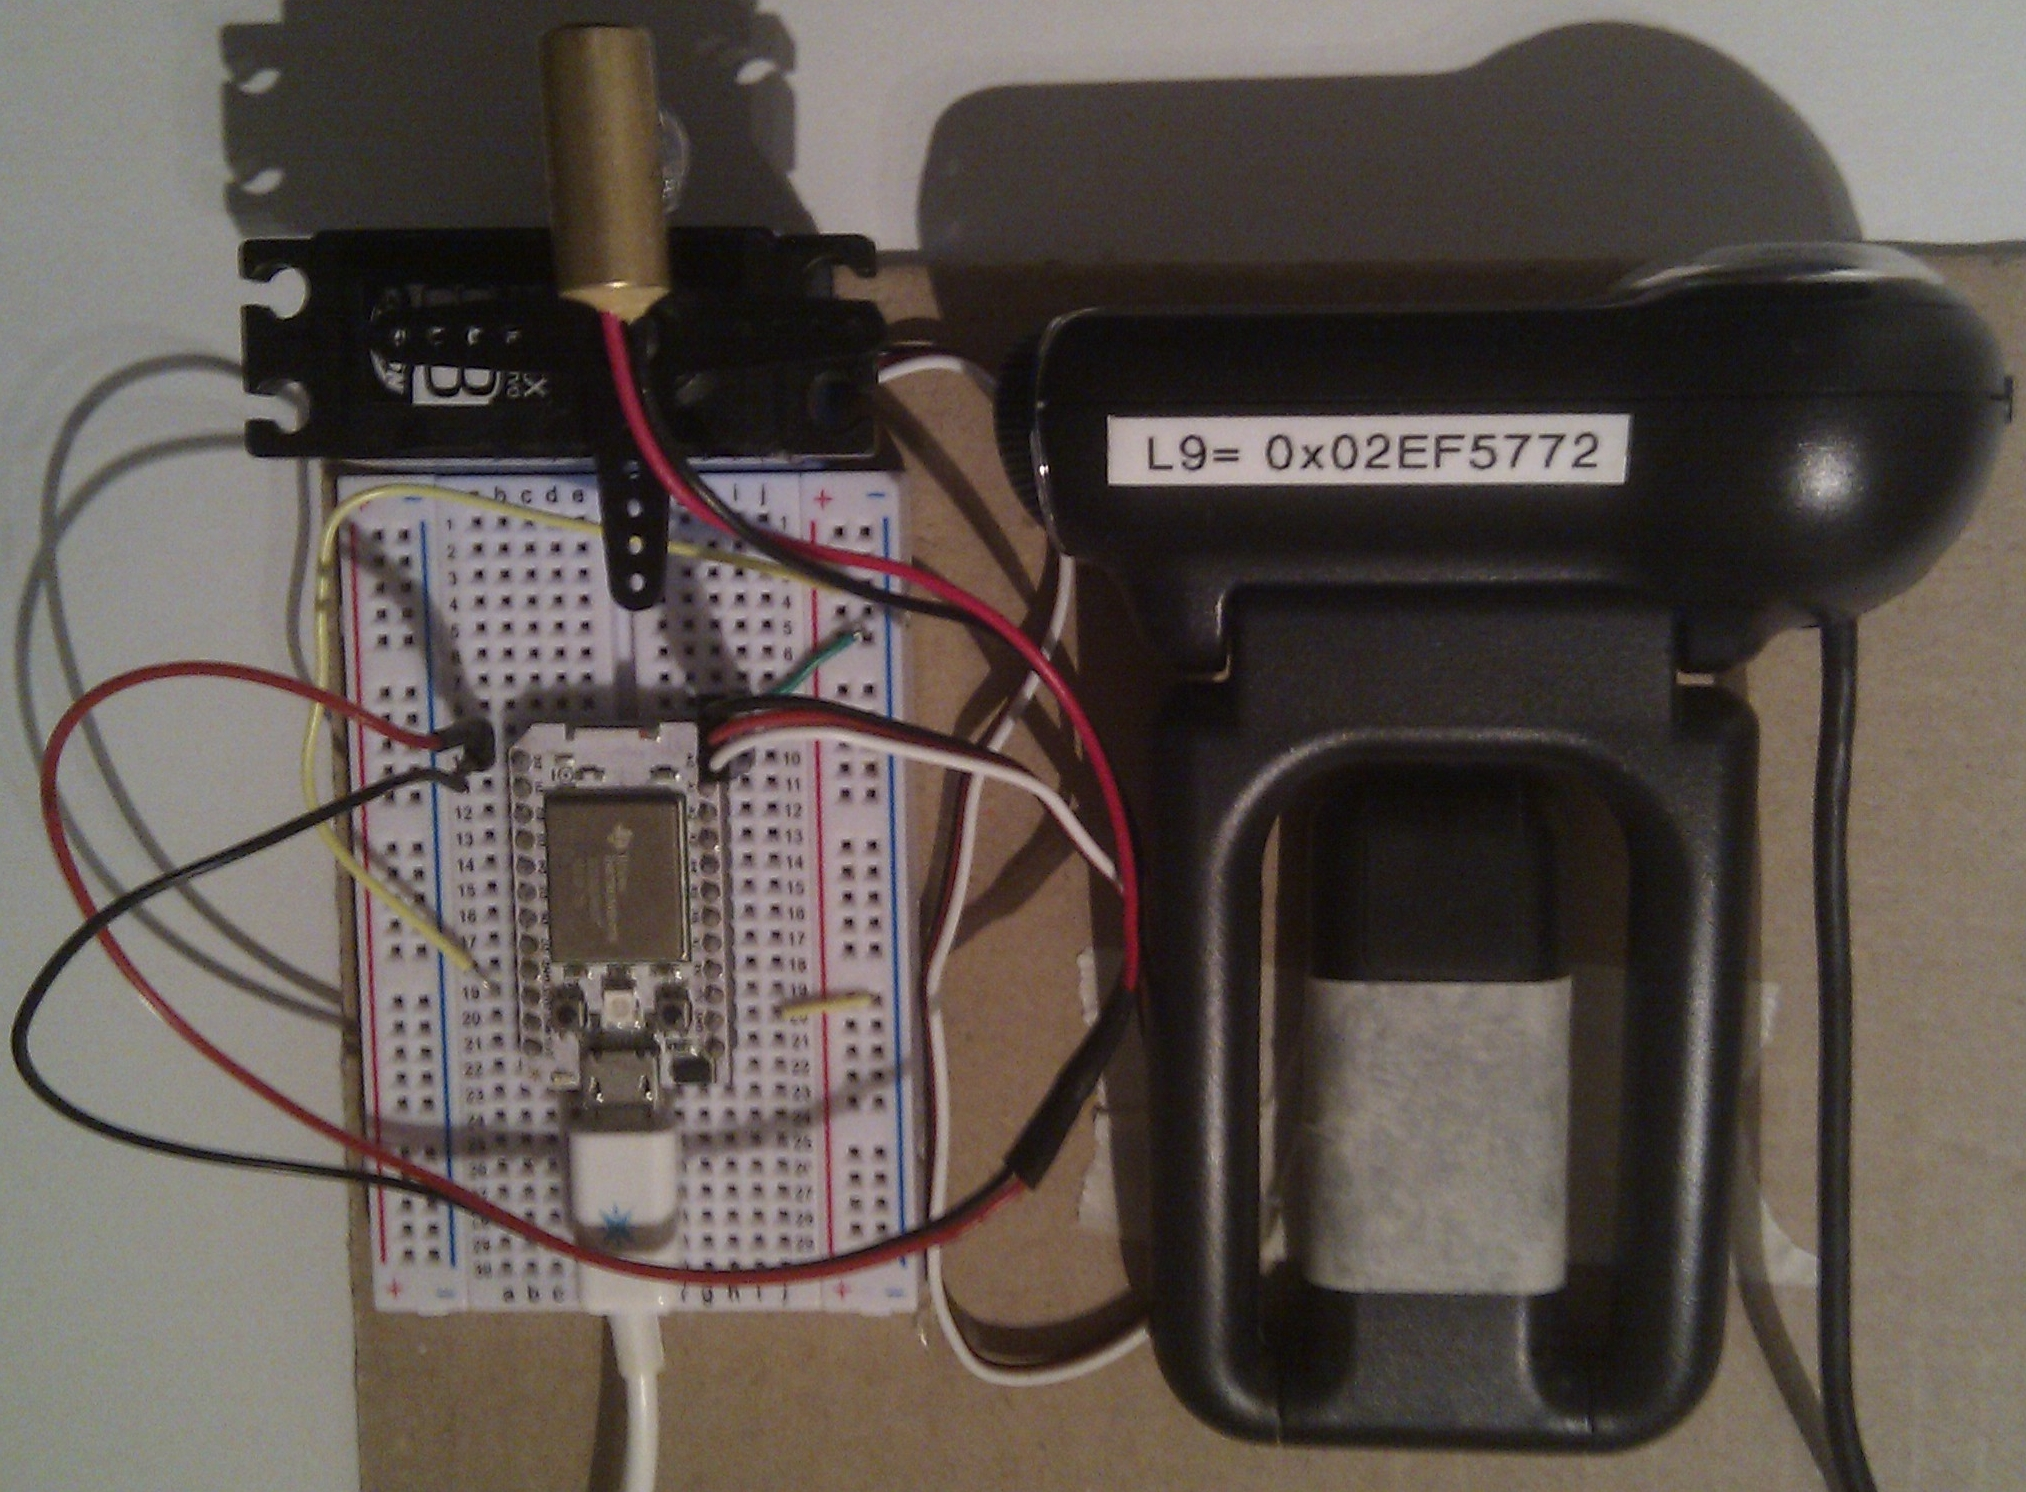
\includegraphics[width=0.9\linewidth]{includes/hardware.jpg}

\end{frame}


%\subsection{Ablauf}
\begin{frame}
	\frametitle{Umsetzung}
	\framesubtitle{Ablauf}

	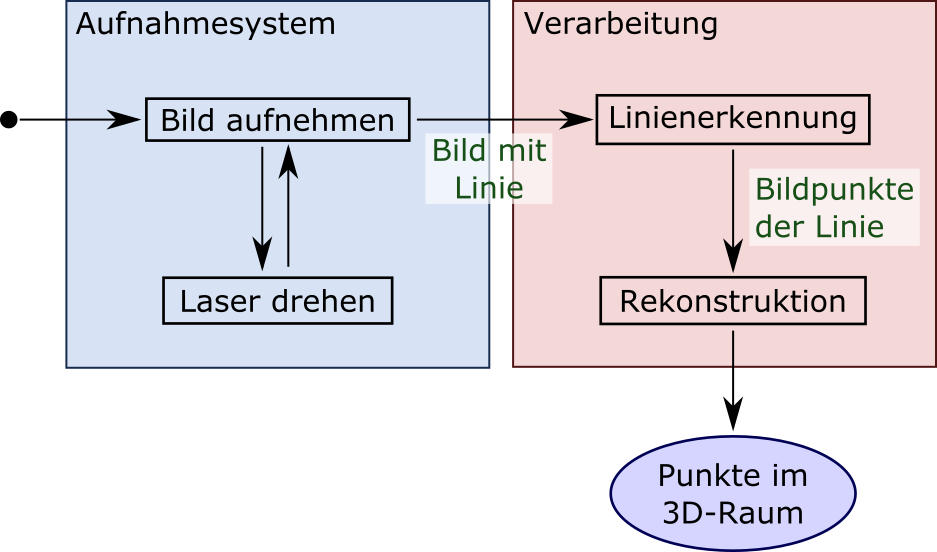
\includegraphics[width=\linewidth]{includes/blockbild.png}

\end{frame}


%\subsection{Linienerkennung}
\begin{frame}
	\frametitle{Umsetzung}
	\framesubtitle{Linienerkennung}

	[TODO]

\end{frame}


%\subsection{Rekonstruktion}
\begin{frame}
	\frametitle{Umsetzung}
	\framesubtitle{Rekonstruktion}

	\begin{columns}
		\small
		\begin{column}{.65\linewidth}
			\begin{itemize}
				\item \textbf{Schritt 1:} Berechne die normalisierten Bildkoordinaten $(u,v)$.
				\item \textbf{Schritt 2:} Bestimme $\alpha$, $\beta$, $c$ und $f$ aus der Gerätekonfiguration und den Bildkoordinaten.
				\item \textbf{Schritt 3:} Berechne $h$:
				\[h = \frac{c * \sin(\alpha) * \sin(\beta)}{\sin(180^\circ - \beta - \alpha)}\]
				\item \textbf{Schritt 4:} Bestimme Koordinaten innerhalb der Szene.
				\[\begin{pmatrix}x\\y\\z\end{pmatrix} = \frac{h}{f} *
				\begin{pmatrix}u\\v\\-f\end{pmatrix}\]
			\end{itemize}
		\end{column}
		\begin{column}{.35\linewidth}
			\hfill\fbox{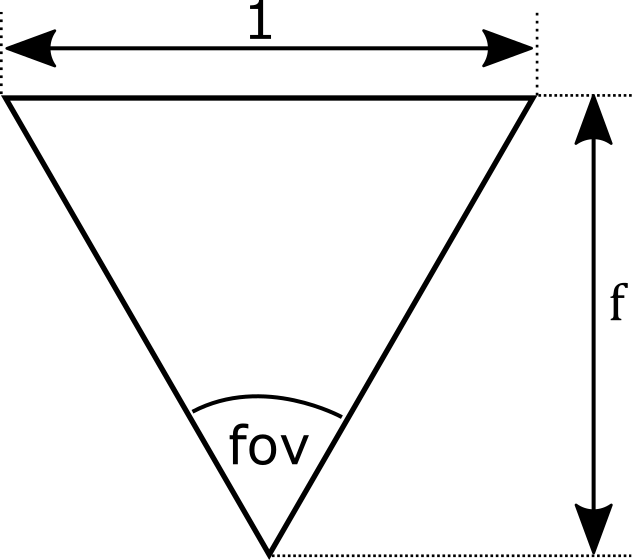
\includegraphics[width=0.9\linewidth]{includes/reconstruction_2}}
			\vfill\vspace{4ex}\vfill
			\hfill\fbox{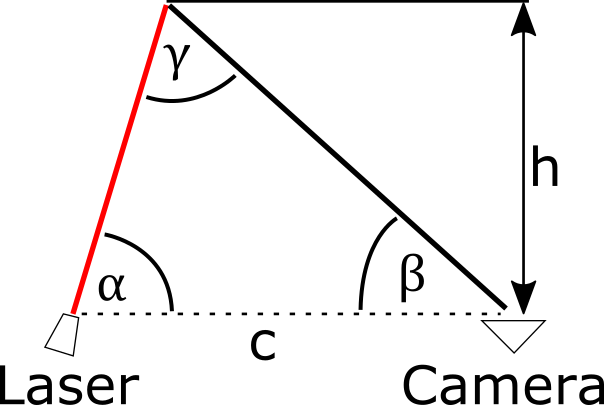
\includegraphics[width=0.9\linewidth]{includes/reconstruction_1}}
		\end{column}
	\end{columns}

\end{frame}


\begin{frame}
	\frametitle{Umsetzung}

	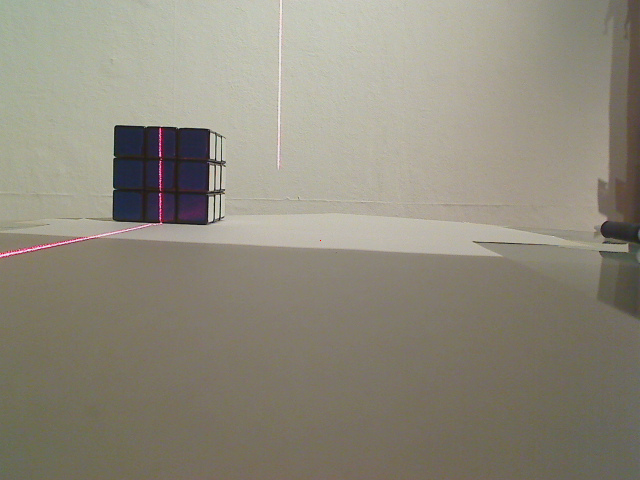
\includegraphics[width=0.9\linewidth]{includes/cap.png}

\end{frame}
\begin{frame}
	\frametitle{Umsetzung}

	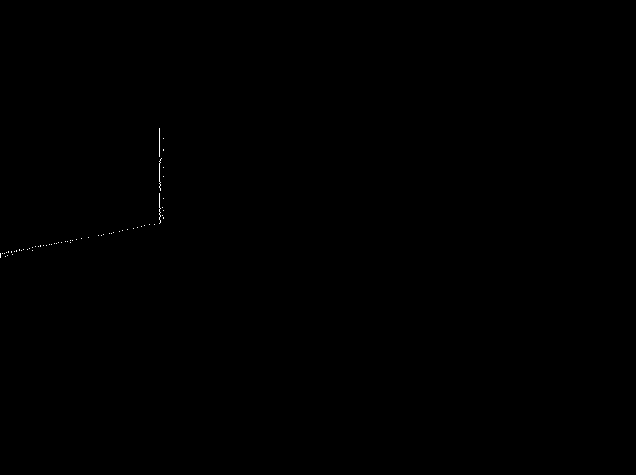
\includegraphics[width=0.9\linewidth]{includes/line.png}

\end{frame}
\begin{frame}
	\frametitle{Umsetzung}

	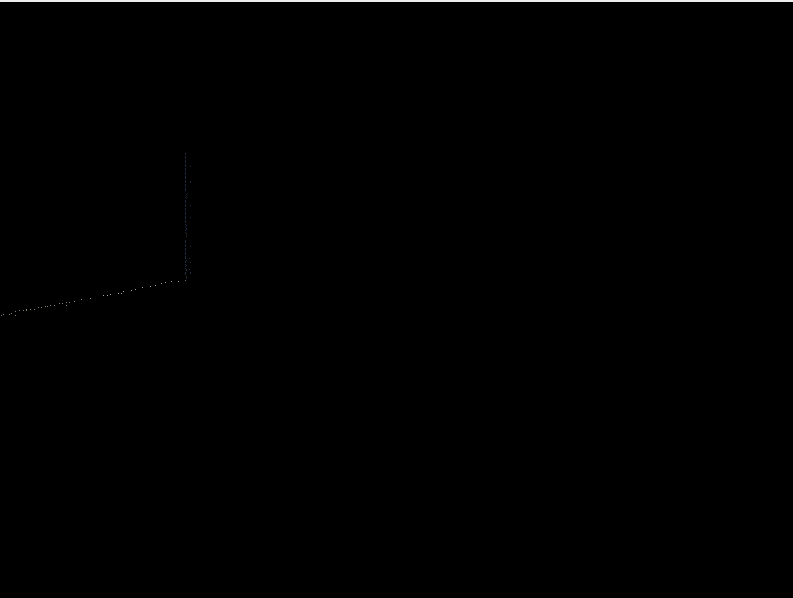
\includegraphics[width=0.9\linewidth]{includes/3d.png}

\end{frame}
\begin{frame}
	\frametitle{Umsetzung}

	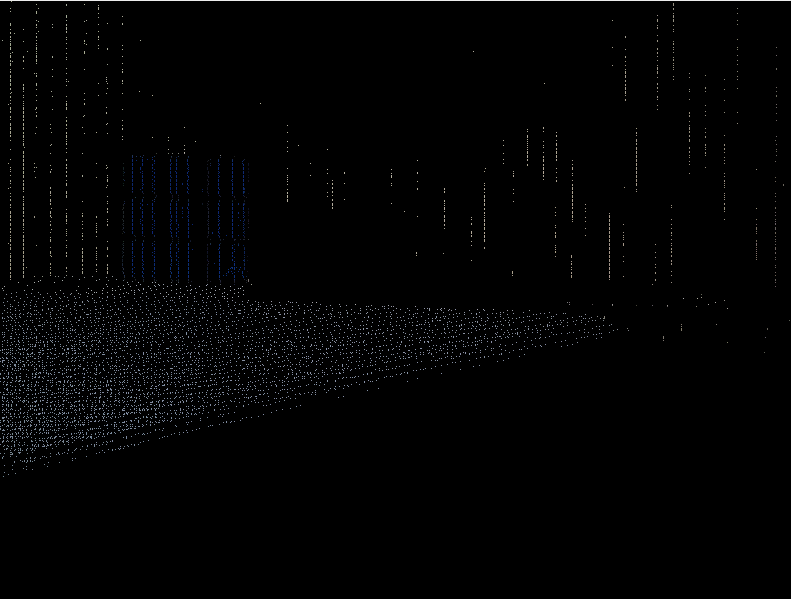
\includegraphics[width=0.9\linewidth]{includes/3d_2.png}

\end{frame}
\begin{frame}
	\frametitle{Umsetzung}

	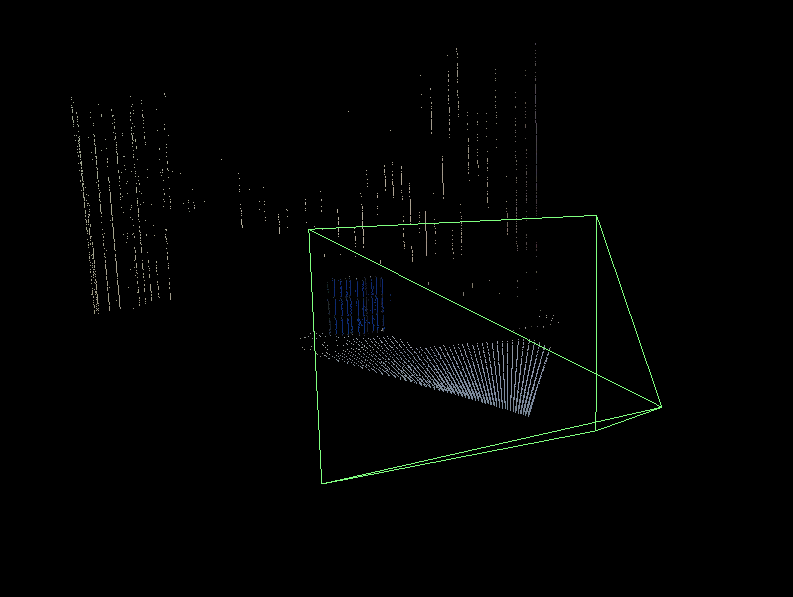
\includegraphics[width=0.9\linewidth]{includes/3d_3.png}

\end{frame}
\begin{frame}
	\frametitle{Umsetzung}

	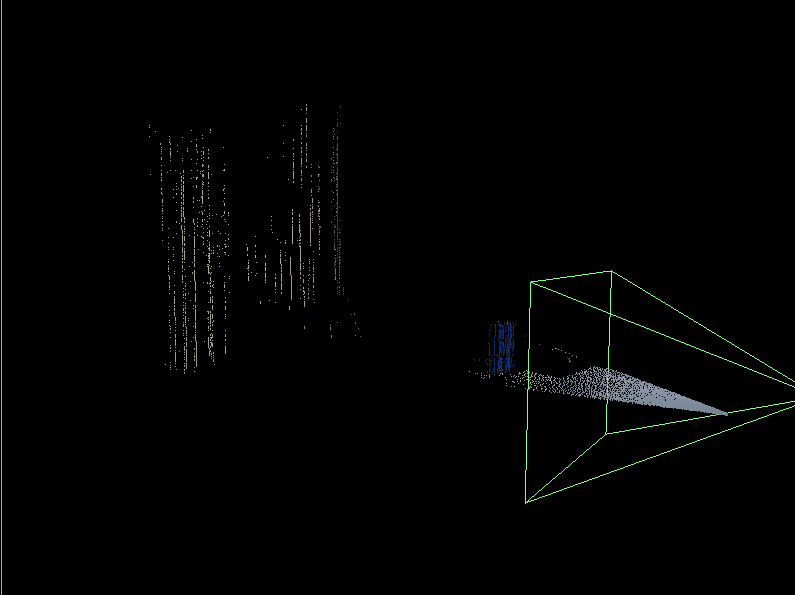
\includegraphics[width=0.9\linewidth]{includes/3d_4.png}

\end{frame}

% ---------------------------------------------------------------------------- %

\section{Probleme}
%\subsection{Organisatorisches}
\begin{frame}
	\frametitle{Probleme}
	\framesubtitle{Organsiatorisches}

	\begin{itemize}
		\item Viel Zeit bei der Planung verloren
		\begin{itemize}
			\item Fehlende Erfahrung bei der Strukturierung solcher Anwendungen
			\item Uneinigkeit bei Schwerpunkten und Verfahren
		\end{itemize}
	\end{itemize}

\end{frame}


%\subsection{Hardware}
\begin{frame}
	\frametitle{Probleme}
	\framesubtitle{Hardware}

	\begin{itemize}
		\item Aufbau der Hardware
		\begin{itemize}
			\item Montage von Laser auf Servo
			\item Montage der Kamera
		\end{itemize}
		\item Ursache für Ungenauigkeiten
		\begin{itemize}
			\item kleine Fehler bei der Montage können u.U. zu großen Fehlern führen
			\item schwer die Winkel und Entfernungen zwischen Kamera, Servo und Laser genau zu messen 
		\end{itemize}
	\end{itemize}

\end{frame}


\begin{frame}
	\frametitle{Probleme}
	\framesubtitle{Hardware}

	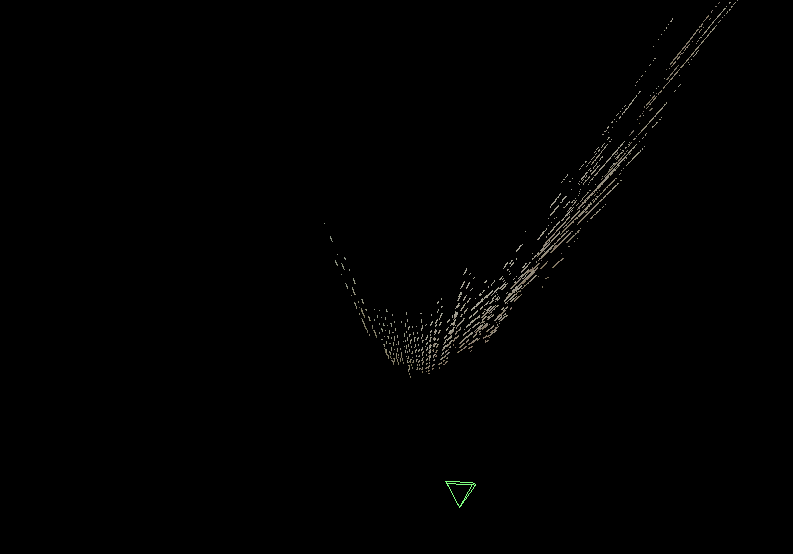
\includegraphics[width=\linewidth]{includes/krumm.png}

\end{frame}


%\subsection{Linienerkennung}
\begin{frame}
	\frametitle{Probleme}
	\framesubtitle{Linienerkennung}

	\begin{itemize}
		\item Lücken
		\item Hintergrundfarbe
	\end{itemize}

\end{frame}

% ---------------------------------------------------------------------------- %

\section{Ergebnisse}
%\subsection{Wiederholte Messungen}
\begin{frame}
	\frametitle{Ergebnisse}
	\framesubtitle{Wiederholte Messungen}

	\begin{figure}
		\begin{minipage}{0.32\linewidth}
			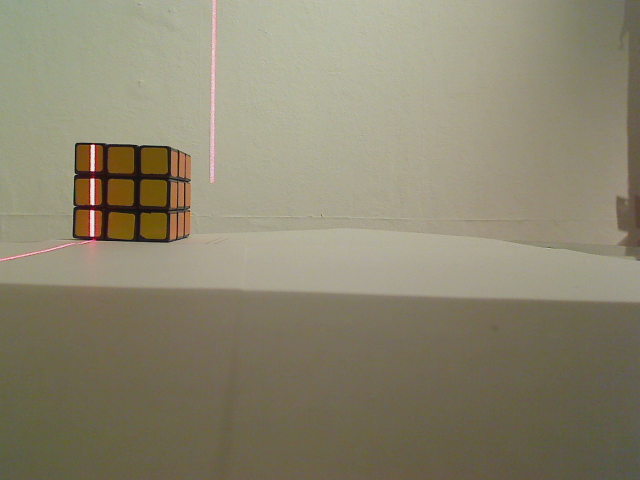
\includegraphics[width=\linewidth]{includes/test_repeat_1}
		\end{minipage}
		\hfill
		\begin{minipage}{0.32\linewidth}
			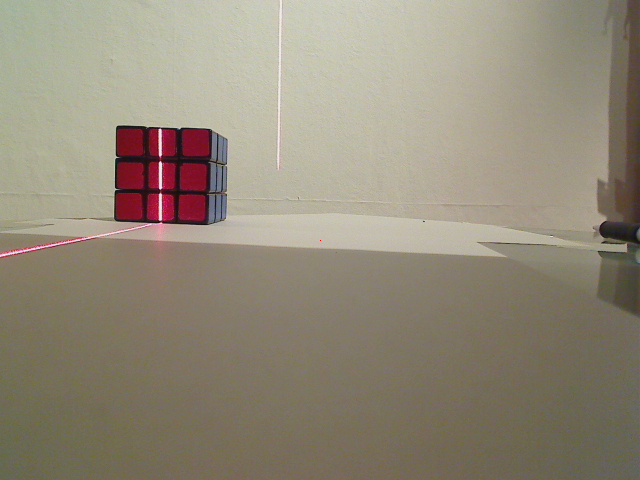
\includegraphics[width=\linewidth]{includes/test_repeat_2}
		\end{minipage}
		\hfill
		\begin{minipage}{0.32\linewidth}
			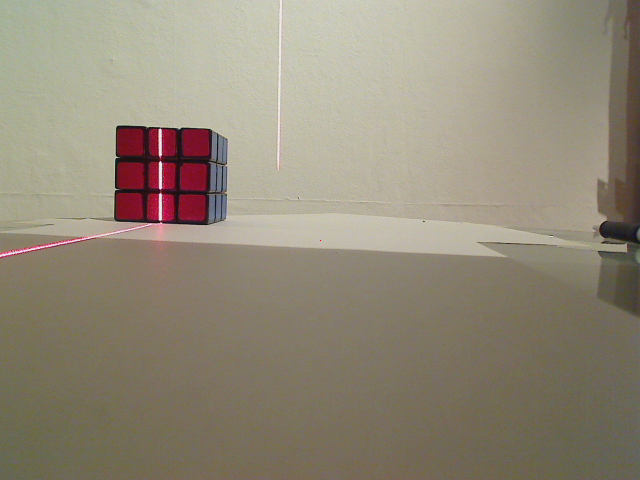
\includegraphics[width=\linewidth]{includes/test_repeat_3}
		\end{minipage}
	\end{figure}

	\begin{onlyenv}<1>
		Reale Höhe: 56mm
		\begin{tabular}{c|c|c|c}
			Messung & Hoehe (mm) & Abw (mm) & Abw (\%) \\
			1 & 54.9 & -1.1 & -1.9\\
			2 & 54.9 & -1.1 & -1.9\\
			3 & 54.9 & -1.1 & -1.9\\
			4 & 54.9 & -1.1 & -1.9\\
			5 & 54.9 & -1.1 & -1.9\\
			6 & 54.9 & -1.1 & -1.9\\	
		\end{tabular}
	\end{onlyenv}
	\begin{onlyenv}<2>
		Reale Entfernung: 300mm 
		\begin{tabular}{c|c|c|c|c|c}
			Messung & Min & Max & Avg & Abw (mm) & Abw (\%)\\
			1 & 307.2 & 316.8 & 314.1 & 14.1 & 4.7\\
			2 & 303.5 & 316.8 & 314.1 & 14.1 & 4.7\\
			3 & 307.2 & 316.8 & 314.1 & 14.1 & 4.7\\
			4 & 309.1 & 316.8 & 314.1 & 14.1 & 4.7\\
			5 & 305.3 & 316.8 & 314.1 & 14.1 & 4.7\\
			6 & 307.2 & 316.8 & 314.1 & 14.1 & 4.7\\
			Stabw  & 0.19157 & 0 & 0.00826 & 0.00826 &0.00027
		\end{tabular}
	\end{onlyenv}

\end{frame}


%\subsection{Verschiedene Farben}
\begin{frame}
	\frametitle{Ergebnisse}
	\framesubtitle{Verschiedene Farben}

	\begin{figure}
		\begin{minipage}{0.32\linewidth}
			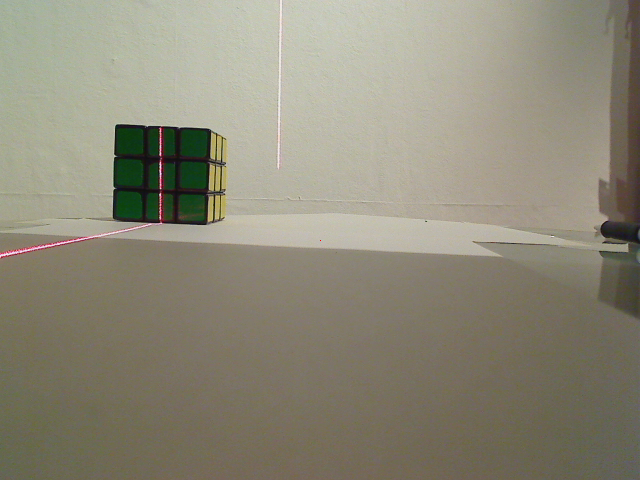
\includegraphics[width=\linewidth]{includes/test_color_1}
		\end{minipage}
		\hfill
		\begin{minipage}{0.32\linewidth}
			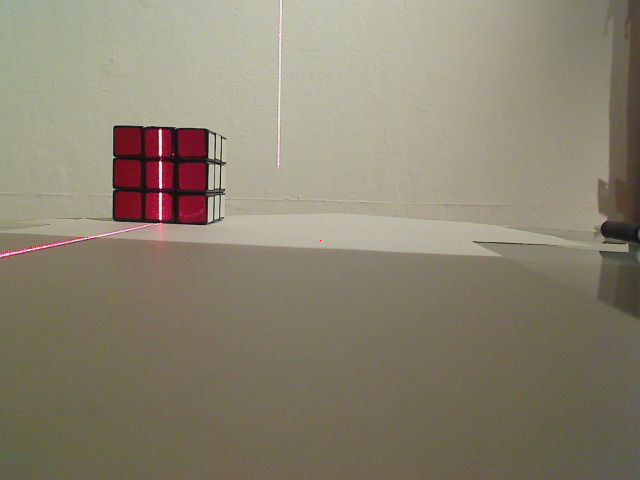
\includegraphics[width=\linewidth]{includes/test_color_2}
		\end{minipage}
		\hfill
		\begin{minipage}{0.32\linewidth}
			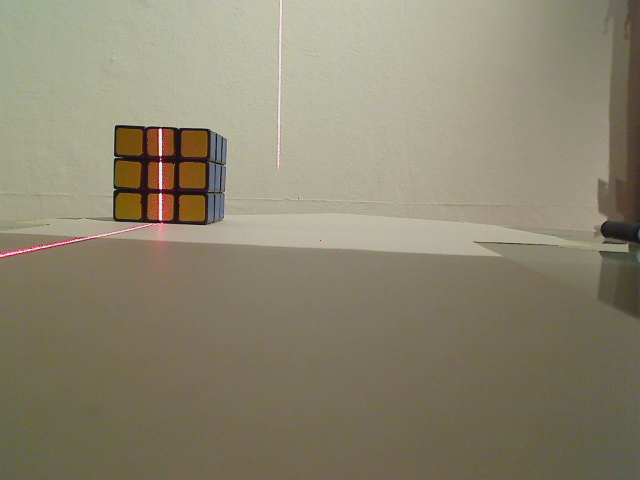
\includegraphics[width=\linewidth]{includes/test_color_3}
		\end{minipage}
	\end{figure}

	\begin{onlyenv}<1>
		Reale Höhe: 56mm
		\begin{tabular}{c|c|c|c}
			Farbe & Hoehe (mm) & Abw (mm) & Abw (\%) \\
			Blau & 55.0 & -1 & -1.8\\
			Grün & 57.0 & 1 & 1.8\\
			Orange & 54.5 & -1.5 & -2.7\\
			Rot & 55.4 & -0.6 & -1.1\\
			Weise & 56.6 & 0.6 & 1.1\\
			Gelb & 54.8 & -1.2 & -2.1	
		\end{tabular}
	\end{onlyenv}
	\begin{onlyenv}<2>
		Reale Entfernung: 300mm 
		\begin{tabular}{c|c|c|c|c|c}
			Farbe & Min & Max & Avg & Abw (mm) & Abw (\%)\\
			Blau & 314.9 & 318.8 & 315.2 & 15.2 & 5.1\\
			Grün & 314.9 & 318.9 & 315.6 & 15.6 & 5.2\\
			Orange & 307.2 & 318.9 & 314.4 & 14.4 & 4.8\\
			Rot & 305.3 & 318.9 & 314.4 & 14.4 & 4.8\\
			Weiß & 298.1 & 316.8 & 310.4 & 10.4 & 3.5\\
			Gelb & 284.7 & 320.9 & 314.0 & 14.0 & 4.7
		\end{tabular}
	\end{onlyenv}

\end{frame}


%\subsection{Verschiedene Entfernungen}
\begin{frame}
	\frametitle{Ergebnisse}
	\framesubtitle{Verschiedene Entfernungen}

	\begin{figure}
		\begin{minipage}{0.32\linewidth}
			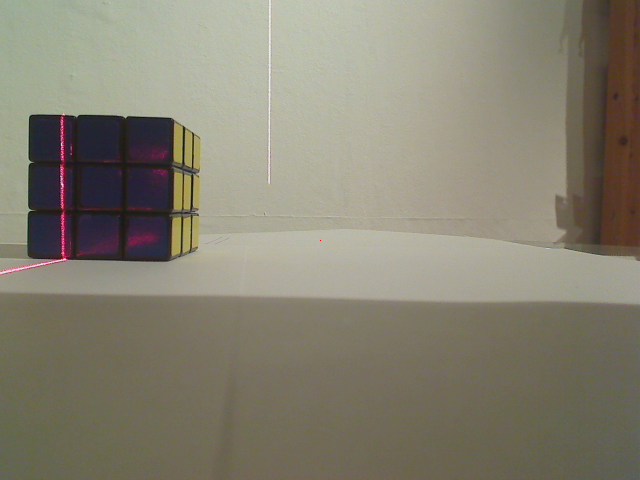
\includegraphics[width=\linewidth]{includes/test_dist_1}
		\end{minipage}
		\hfill
		\begin{minipage}{0.32\linewidth}
			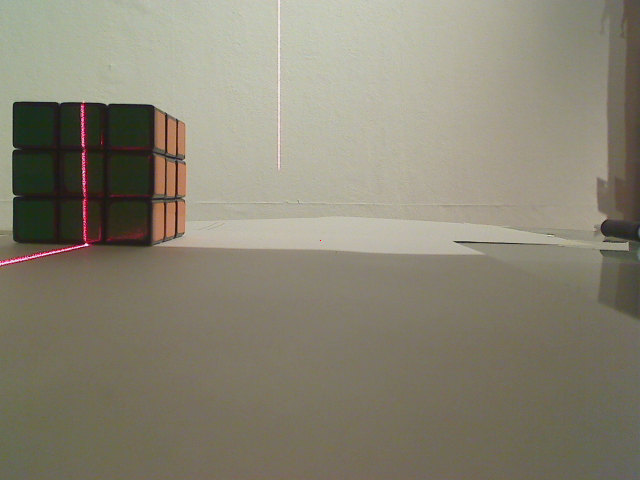
\includegraphics[width=\linewidth]{includes/test_dist_2}
		\end{minipage}
		\hfill
		\begin{minipage}{0.32\linewidth}
			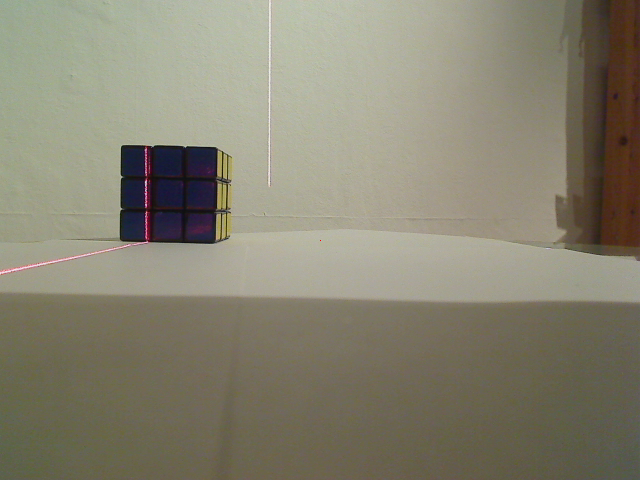
\includegraphics[width=\linewidth]{includes/test_dist_3}
		\end{minipage}
	\end{figure}

	\begin{onlyenv}<1>
		Reale Höhe: 56mm
		\begin{tabular}{c|c|c|c}
			Entfernung & Hoehe & Abw (mm) & Abw (\%) \\
			150 & 57.1.0 & 1.1 & 2.0\\
			200 & 57.1 & 1.1 & 2.0\\
			250 & 57.4 & 1.4 & 2.5\\
			300 & 57.2 & 1.2 & 2.1\\
			350 & 56.4 & 0.4 & 0.7
		\end{tabular}
	\end{onlyenv}
	\begin{onlyenv}<2>
		\begin{tabular}{c|c|c|c|c|c}
			Entfernung & Min & Max & Avg & Abw (mm) & Abw (\%)\\
			150 & 161.2 & 163.3 & 162.1 & 12.1 & 8.0\\
			200 & 211.0 & 215.5 & 212.9 & 12.9 & 6.5\\
			250 & 262.5 & 268.1 & 263.8 & 13.8 & 5.5\\
			300 & 316.8 & 320.9 & 317.6 & 17.6 & 5.9\\
			350 & 335.8 & 373.0 & 369.9 & 19.9 & 5.7
		\end{tabular}
	\end{onlyenv}

\end{frame}

% ---------------------------------------------------------------------------- %

\section{Ausblick}
\begin{frame}
	\frametitle{Ausblick}

	\begin{itemize}
		\item Fehler durch bessere Kalibrierung und/oder besseres Setup minimieren
		\item Linienerkennung (ohne Referenzbild) robuster gestalten
		\item Objekt statt Kamera bewegen
	\end{itemize}

\end{frame}

% ---------------------------------------------------------------------------- %

\section{Live-Demo} 
\begin{frame}
	\frametitle{Live-Demo}
\end{frame}

% ---------------------------------------------------------------------------- %

\section{Quellen} 
\begin{frame}
	\frametitle{Quellen}

\end{frame}


\end{document}
